% !TEX root = ../main.tex

\chapter{Technical execution} % (fold)
\label{chp:execution}

\section{Organising state} % (fold)
\label{sec:organising_state}

talk about the difference between storing params and storing widgets

% section organising_state (end)

\section{Handling state changes} % (fold)
\label{sec:handling_state_changes}

Research:

\begin{itemize}
  \item observables vs flux
  \item Other languages (Elm model)
\end{itemize}

% section handling_state_changes (end)

\section{Getting responses from the API} % (fold)
\label{sec:getting_responses_from_the_api}

% section getting_responses_from_the_api (end)

\section{Rendering refinements} % (fold)
\label{sec:rendering_refinements}


% section rendering_refinements (end)

\section{Overview} % (fold)
\label{sec:overview}

\begin{figure}[H]
  \label{figure:company-logo}
  \centering
  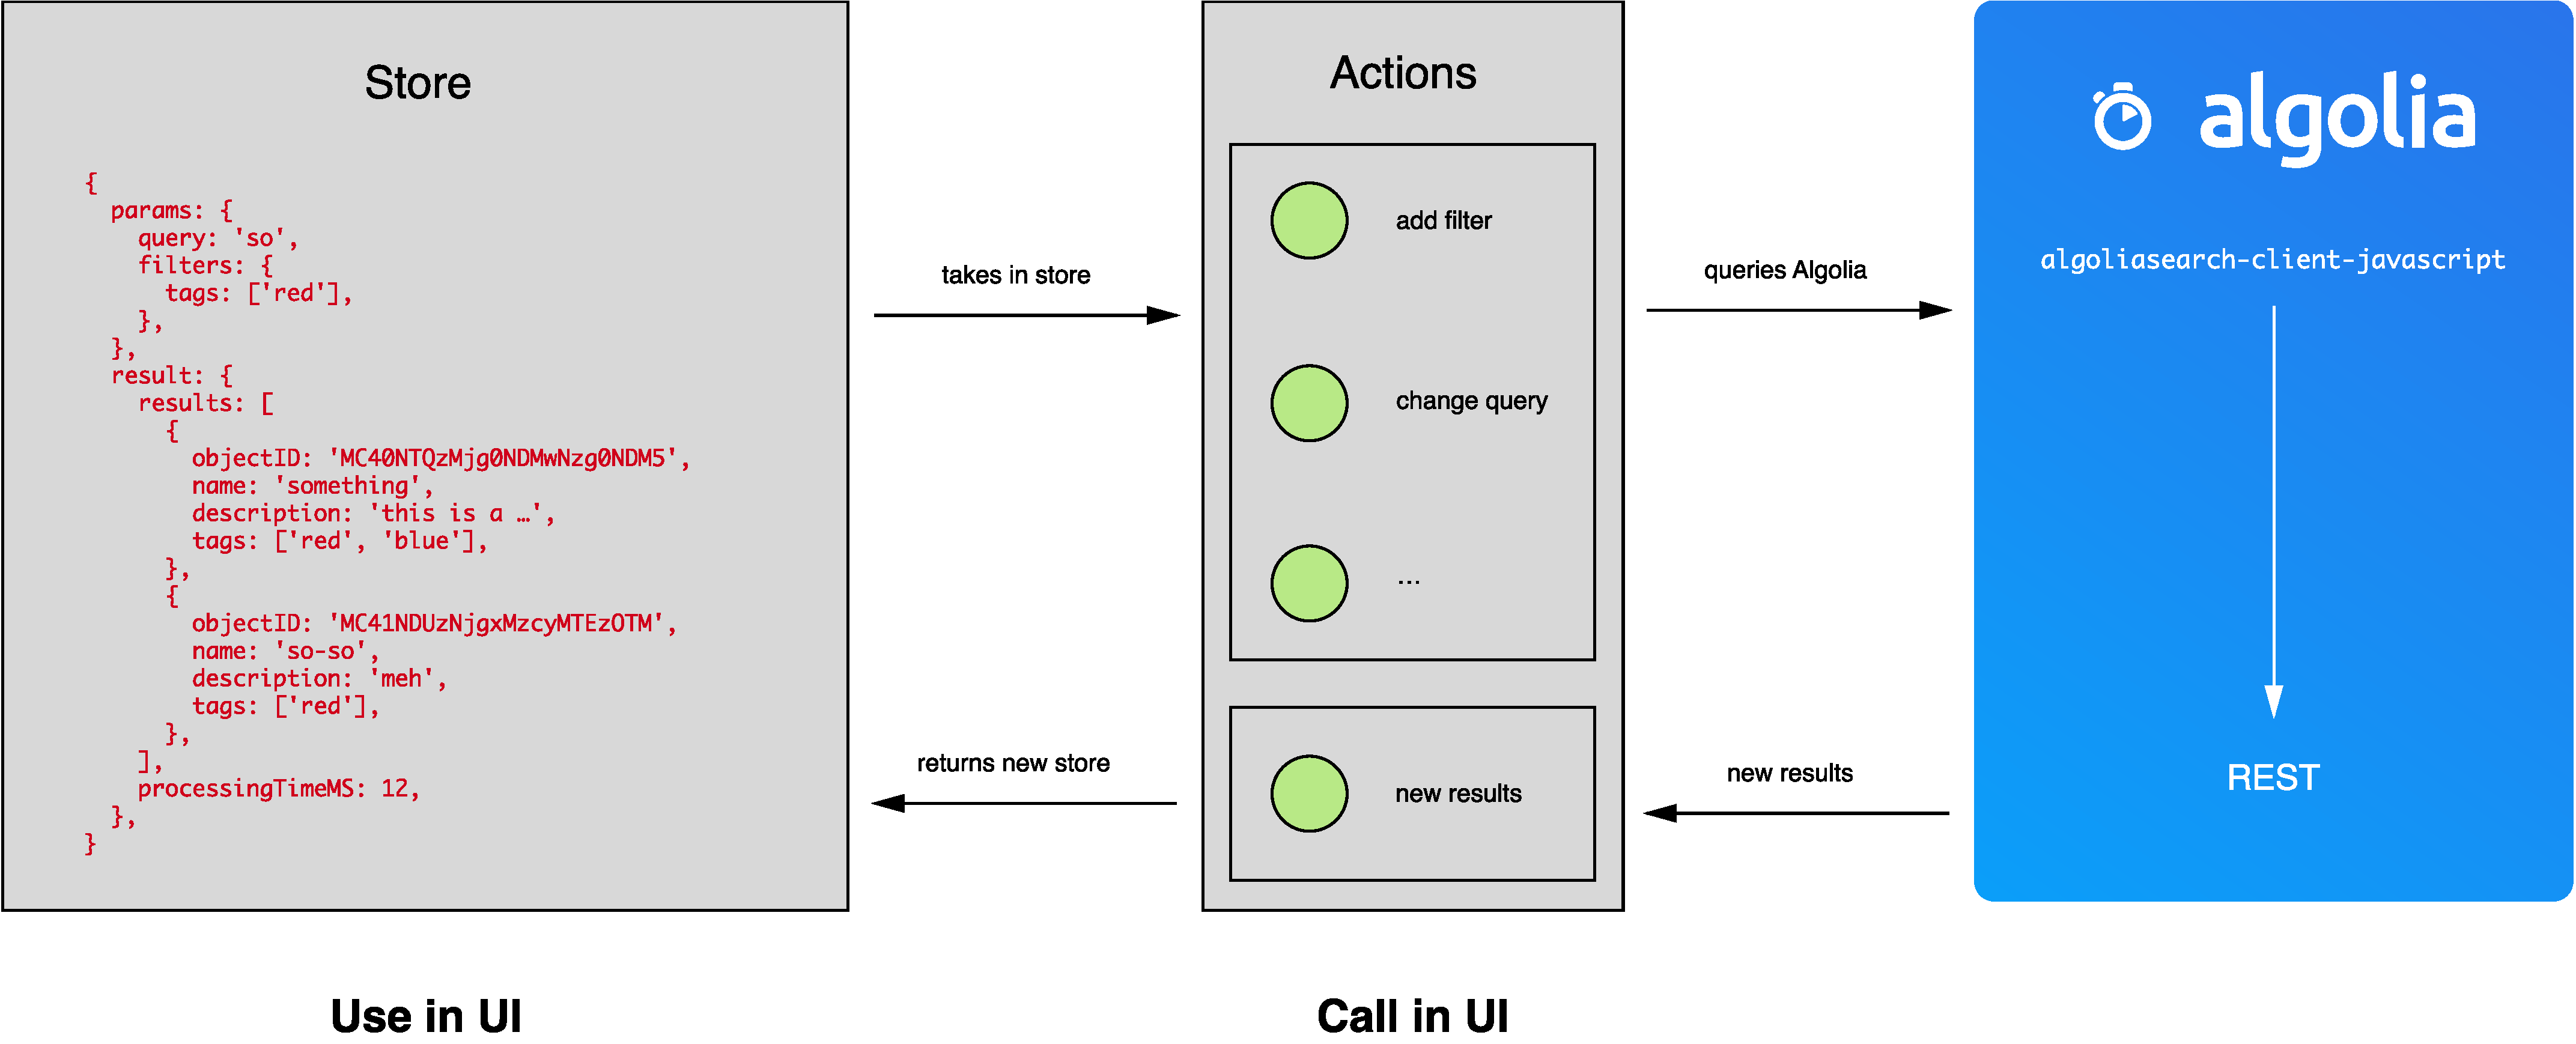
\includegraphics[width=\textwidth]{../assets/architecture.pdf}
  \caption{Architecture overview\cite{blog-architecture}}
\end{figure}

% section overview (end)

\section{Complete implementation} % (fold)
\label{sec:complete_implementation}


\begin{lstlisting}[caption={Using instantearch-core},label={lst:is-core-usage}]
// stores.js
import algoliasearch from 'algoliasearch';
import { createStore } from 'instantsearch-core';

const appId = 'OFCNCOG2CU';
const apiKey = 'f54e21fa3a2a0160595bb058179bfb1e';
const indexName = 'products_asc';

const client = algoliasearch(appId, apiKey);
const productsStore = createStore(client, indexName);

export productsStore;

// widget.js
import { setQuery } from 'instantsearch-core/actions/query';
import { productsStore } from './stores';

function onInput(event) {
  event.preventDefault();

  productsStore.refine(setQuery(event.target.value));
}
\end{lstlisting}

% section complete_implementation (end)

